\section{Polar Coordinates}\label{Polar}
We use the \emph{(horizontal,vertical)} coordinate system so much that it is easy to think that it is somehow inherent to a plane.  However, a plane is just a geometric object; a coordinate system is an arbitrary system of labels that we slap on after the fact. Here we explore a different commonly used coordinate system, \emph{polar coordinates}.

\subsection{Points in Polar Coordinates}
Assume we chose an origin in the plane, a direction that we call the positive $x$-axis, and some point along that ray that marks off unit distance.  We now define coordinates for the rest of the plane based on these choices.  

\begin{definition}{\polar{Plotting Points} in Polar Coordinates} The point $(\theta, r)$ is the point located at an angle $\theta$ radians counterclockwise from the positive $x$-axis, a distance of $r$ units from the origin.  

	\begin{center}
		\includegraphics[width=160pt]{ChapterCalcIII/Figures/polargraph.eps}
	\end{center}

\end{definition}
%JMA: This fig might be better suited inside the grey box. :AMJ
%KMM: Agreed!  Moved.  Can we get a little bracey thing showing the segment r is labeling the measure of?

Notice the angles are measured in the same manner as on the unit circle in trigonometry.  The difference here is we allow any real number $r$ as radius, rather than only radius one.  We do allow $r$ to be a negative number, in which case we travel ``backwards'' along the ray given by $\theta$.

\begin{example}{Polar Coordinates are not Unique!}
Be warned that any given point will have many different representations in polar coordinates.  For example, consider the cartesian point (1,-1).  In polar coordinates, we have many ways to represent this point.  We can think of the angle as $\theta=-\pi/4$ and the radius as $r=\sqrt{2}$.  We can also think of the angle as $\theta=7\pi/4$ and the radius as $r=\sqrt{2}$.  Yet another valid way to reach that same point is to use angle $\theta=3\pi/4$ and the radius $r=-\sqrt{2}$.  Thus, in polar coordinates we have that $$\left(-\pi/4,\sqrt{2}\right)=\left(7\pi/4,\sqrt{2}\right)=\left(3\pi/4,-\sqrt{2}\right) $$ all represent the same point.
\end{example}

We now see how right-triangle trigonometry allows us to convert between polar coordinates and cartesian coordinates.

\begin{exercise}{\polar{Converting Between Polar and Cartesian} \Coffeecup \Coffeecup \Coffeecup}\label{convertingPolar}
\begin{itemize}
\item See the diagram below, with a point in QI labeled with both cartesian and polar measurements.  For each of the conversion formulas listed below, write a short sentence afterwards explaining how it comes from the diagram.
	\begin{center}
	\begin{tabular}{c c}
    \includegraphics[width=130pt]{ChapterCalcIII/Figures/QITri.eps} &
    \includegraphics[width=130pt]{ChapterCalcIII/Figures/QIPolar.eps}
	\end{tabular}
    \end{center}

\begin{itemize}
\item $x^2+y^2=r^2$
\item $x=r\cos(\theta)$
\item $y=r\sin(\theta)$
\item $\tan(\theta)=\frac{y}{x}$
\item $\theta = \arctan\left(\frac{y}{x}\right)$
\end{itemize} 

\item If the point of interest were in a different quadrant, do the above formulas still hold?  Do any of them require adjustment?  Explain.
\vspace*{1in}
\end{itemize}
\end{exercise}

\begin{exercise}{Plotting in Polar \Coffeecup \Coffeecup}
\begin{itemize}
\item Plot the polar point ($5\pi/4$,4).  What are its cartesian coordinates?
\vspace*{1in}
\item Consider the cartesian point (2,0).  What are \emph{all} possible ways of writing that point in polar coordinates?
\vspace*{1in}
\end{itemize}
\end{exercise}

\begin{exercise}{Do Any Points Have the Same Name? \Coffeecup \Coffeecup \Coffeecup }
Do any points happen to have the same label in both polar and cartesian coordinates?  Find all points that do, and explain why there are no more!  \vspace*{.5in}
\end{exercise}

It is worth noting why ``polar coordinates'' are called what they are called.  Cartesian coordinates look like a grid of horizontal and vertical lines.  This is a great approximation of what latitude and longitude lines look like if you are standing at a random point on earth and think of your surroundings as approximated by a plane.  But, if you are standing at the north or south pole, the latitude and longitude lines do not in any way look like a grid!

\begin{exercise}{Justifying the Name \Coffeecup \Coffeecup}
What do the lattitude and longitutde lines look like if you are standing at the north or south pole?  Draw a small graph below.  \vspace*{.5in}
\end{exercise}

\begin{exercise}{The Idea of Coordinate Systems \Coffeecup \Coffeecup \Coffeecup \Coffeecup}
Create another coordinate system for the plane that is not cartesian and is not polar!  Describe your system of labeling all the points!
\vspace*{1in}
\end{exercise}

\subsection{\polar{Graphs of Equations and Functions} in Polar Coordinates}

An equation in \graphing{polar coordinates} is an equality between expressions involving $r$ and $\theta$.  We often wish to view the solutions visually by plotting all points $\left(\theta, r\right)$ in the plane that make the equations true (just as one would in cartesian). 

\begin{example}{Graphing a Polar Equation}
Suppose we wish to graph the equation $$\theta=\pi/3 $$
A point satisfies that equation if and only if the angle is $\pi/3$.  The radius $r$ is free to be any real number -positive, negative, or zero.  For example, points that satisfy the equation include $(\pi/3,1), (\pi/3,0),$ and $(\pi/3,-1)$.  Thus the graph is a line through the origin at $60^\circ$ to the positive $x$-axis.


	\begin{center}
		\includegraphics[width=185pt]{ChapterCalcIII/Figures/linepolargraph.eps}
	\end{center}
\end{example}

\begin{exercise}{Graphing Equations \Coffeecup \Coffeecup }
Graph the following equations.

\begin{itemize}
\item $r=2$
	\begin{center}
		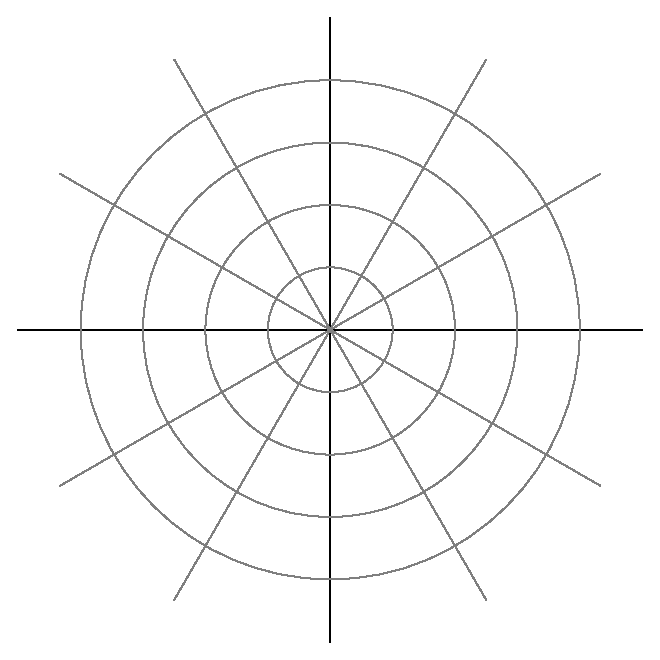
\includegraphics[width=150pt]{polar.eps}
	\end{center}
\item $r=-2$
	\begin{center}
		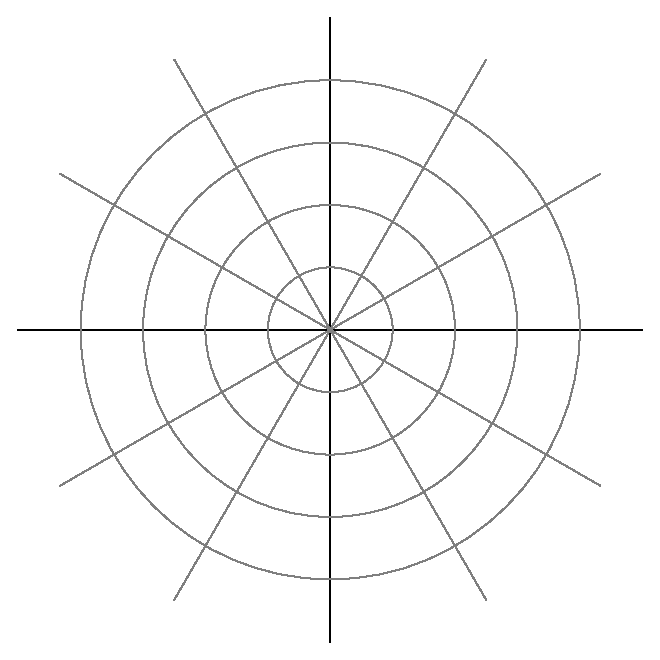
\includegraphics[width=150pt]{polar.eps}
	\end{center}
\item $\theta^2=\pi^2/4$
	\begin{center}
		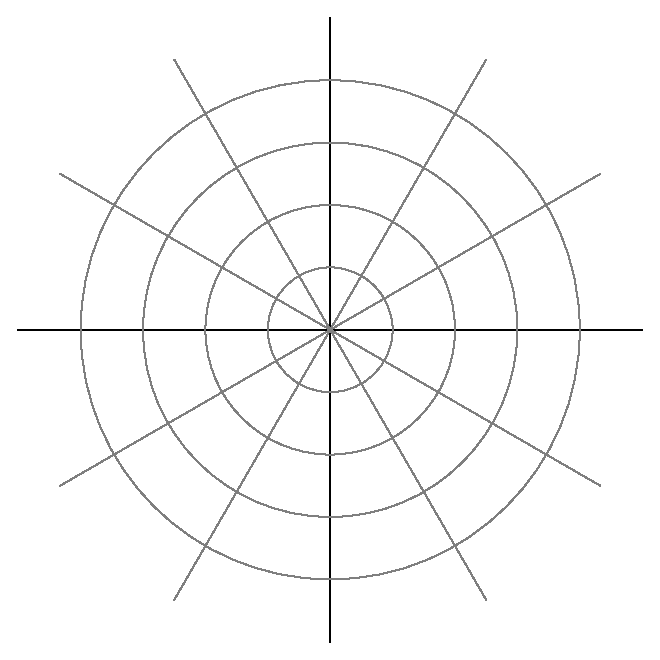
\includegraphics[width=150pt]{polar.eps}
	\end{center}
\end{itemize}
\end{exercise}

If the equation can be solved for $r$, we can consider $r$ as a function of the independent variable $\theta$.  To graph a function, we simply make an input-output table of $\theta$ values and corresponding $r(\theta)$ values and plot the corresponding points $\left( \theta , r(\theta)\right)$.

\begin{example}{Graphing a Polar Function}
Plot the polar function $$r(\theta)=\tan(\theta) $$ over the domain $-\pi/2<\theta < \pi/2$.  We select input values for $\theta$ that are clean unit circle values to plot.
\begin{center}
\begin{tabular}{|c||c|c|c|c|c|c|c|c|c|} \hline
$\theta$ & $ -\pi/2$ &$ -\pi/3$ &$ -\pi/4$  &$-\pi/6$ & 0 & $\pi/6$ & $\pi/4$ &$\pi/3$ &$\pi/2$ \\ \hline
$r(\theta)$ & $ DNE $ &$ -\sqrt{3}$ &$ -1$  &$-\sqrt{3}/3$ & 0 & $\sqrt{3}/3 $ & $1$ &$\sqrt{3}$ &$DNE$ \\ \hline
\end{tabular}
\end{center}

	\begin{center}
		\includegraphics[width=175pt]{ChapterCalcIII/Figures/tanpolar.eps}
	\end{center}
\end{example}

\begin{exercise}{Analyzing the Graph  \Coffeecup \Coffeecup}
Does the graph appear to have any asymptotes?  If so, where?
\vspace*{.5in}
\end{exercise}

Looking at the graph prompts the question ``can we find a Cartesian equation that describes the same set of points''?  Here we use the formulas from Exercise \ref{Polar}.\ref{convertingPolar} to rewrite all instances of $r$ and $\theta$ in terms of $x$ and $y$.  Also, perhaps the cartesian equation can confirm our asymptote suspicions above!

\begin{example}{Converting to Cartesian} Let's find a cartesian equation for the graph of $r(\theta)=\tan(\theta) $ from the previous example.  Since we do not have a particularly clean conversion formula for $r$ itself but rather for $r^2$, it can be helpful to either multiply both sides by $r$ or square both sides.  In this case, squaring both sides will be cleaner so we take that path.  Proceeding:
\begin{align*}
r&=\tan(\theta) \\
r^2&=\left(\tan(\theta)\right)^2 \\
x^2+y^2&=\left(\frac{y}{x}\right)^2 \\
x^2+y^2&=\left(\frac{y}{x}\right)^2  \\
x^4+x^2y^2&=y^2  \\
x^4+\left(x^2-1\right)y^2&=0  \\
y^2&=\frac{x^4}{1-x^2}  \\
y&=\pm \frac{x^2}{\sqrt{1-x^2}} \\
\end{align*}
\end{example}

\begin{exercise}{Analyzing the Graph, Round II \Coffeecup \Coffeecup}
Does the cartesian formula tell you anything further about the apparent asymptotes on the graph?
\vspace*{.5in}
\end{exercise}
The next exercise shows why converting \circles{a polar graph} to cartesian coordinates can help analyze the geometry of the graph.
\begin{exercise}{Graphing a Function and Converting \Coffeecup \Coffeecup \Coffeecup}
\begin{itemize}
\item Graph the function $r(\theta)=\sin(\theta)$.  Does it look like a circle?
	\begin{center}
	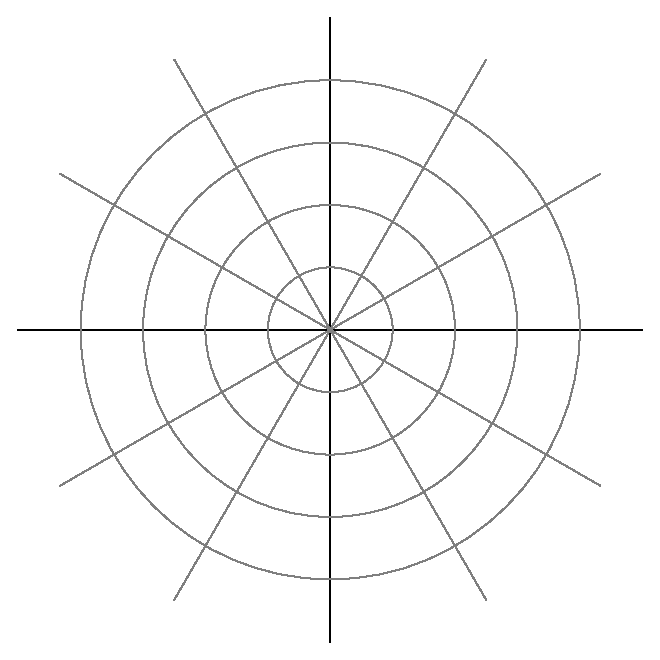
\includegraphics[width=150pt]{polar.eps}
    \end{center}

\item Is it a circle?  If so, what is the center and radius?  Convert the equation to cartesian coordinates to confirm!   
\vspace*{1in}
\end{itemize}
\AnswerKeyEntry{Yes, it is in fact a circle with cartesian center $\left(0,1/2\right)$ and radius 1/2.  This can be verified by demonstrating the polar equation converts to the cartesian equation $$x^2+\left(y-\frac{1}{2}\right)^2=\left(\frac{1}{2}\right)^2. $$}
\end{exercise}

\section{\polar{Derivatives} in \tangentline{Polar Coordinates}}
Suppose we have the graph of a \deriv{polar function} $r(\theta)$, and we would like to find the slope of the tangent line at a point.  We can consider this graph to be a parameterized curve by treating $t=\theta$ as the parameter.  Specifically, the parameterization is given by

\begin{center}
\begin{align*}
x(t)&=r(t)\cos(t)\\
y(t)&=r(t)\sin(t).
\end{align*}
\end{center}

\begin{exercise}{Deriving the Derivative \Coffeecup \Coffeecup}
Use the formula for the derivative of a parametric curve to find the formula for the \parametric{derivative of a polar graph}. \vspace*{1in} 
\end{exercise}

\begin{exercise}{Using the Formula \Coffeecup \Coffeecup}
Use the polar derivative formula above to find the slope of the graph of $r(\theta)=\sec(\theta)$.  What does this let you conclude about that graph? \vspace*{2in}
\AnswerKeyEntry{The derivative is a constant; thus the graph is a straight line!}
\end{exercise}

\section{Area in Polar Coordinates}

To compute \polar{area} in polar coordinates, we essentially repeat the process of taking a Riemann sum.  Rather than using rectangles however, we use sectors of circles. 

\begin{exercise}{Area of a Single Sector \Coffeecup \Coffeecup}
\begin{itemize}
\item What is the area of an entire circle with radius $r$?  Draw the circle.  \vspace*{.5in}
\item Within your circle, draw a sector of that circle with angle $\theta$.  What proportion of the area of the entire circle does that sector occupy? \vspace*{.5in}
\item Explain why the area of that sector is $A=\frac{1}{2}r^2\theta.$ \vspace*{.5in}
\end{itemize}
\end{exercise}

We now repeat the process of taking a Riemann sum using sectors of circles.  In particular, say we wish to find the area under the graph of $r(\theta)$ between two rays specified by angles $\theta =\alpha$ and $\theta = \beta $.
\begin{wrapfigure}[8]{r}{0.5\textwidth}
	\begin{center}
		\includegraphics[width=220pt]{ChapterCalcIII/Figures/polararea.eps}
	\end{center}
\end{wrapfigure}

Let $\theta_0,\theta_1,\theta_2,\ldots,\theta_n$ be equally spaced angles from $\alpha$ to $\beta$.  That is, $\theta_0=\alpha$, $\theta_n=b$, and for each $i\in\lbrace 0,1,2,\ldots , n-1 \rbrace$, $\Delta \theta = \theta_{i+1}-\theta_{i}=\frac{\beta-\alpha}{n}$.
\begin{align*}
A&=\lim_{n\rightarrow \infty}\sum_{i=0}^{n-1} \frac{1}{2}r^2\left( \theta_i  \right) \Delta \theta \\
&=\frac{1}{2}\lim_{n\rightarrow \infty}\sum_{i=0}^{n-1}r^2\left( \theta_i  \right) \Delta \theta \\
&=\frac{1}{2}\int_{\theta=\alpha}^{\theta=\beta} r^2(\theta) \dif \theta
\end{align*}

Thus, we have the formula for \integ{polar area}!\\
\vspace*{.7in} %Pushes Theorem out of the wrap

\begin{theorem}{Polar Area}
The \integ{area under a polar curve} $r(\theta)$ between $\theta=\alpha$ and $\theta=\beta$ is $$A=\frac{1}{2}\int_{\theta=\alpha}^{\theta=\beta} r^2(\theta) \dif \theta $$ 
\end{theorem}
Sometimes a helpful way to remember the above formula is to write it as
$$A=\int_{\theta=\alpha}^{\theta=\beta} \pi r^2(\theta) \frac{\dif \theta}{2\pi}. $$

This way you can think of the integrand as the area of a circle being multiplied by what ratio of $2\pi$ radians the change in $\theta$ is occupying.  Canceling the two $\pi$'s and pulling the $\frac{1}{2}$ outside of the integral lands you back at the Polar Area formula.

\begin{exercise}{Looking for Patterns \Coffeecup \Coffeecup \Coffeecup}
Fill out the table! Carry out the instructions listed below for each given value of $n$. 
\begin{itemize}

\item Plot the graph of $r(\theta). $
\item Find the area inside just one ``petal''.
\item What patterns in $n$ do you see?  What can you say about the percent of the unit circle that lies inside rather than outside the graph?
\end{itemize}\begin{center}
\begin{tabular}{|c|c|c|} \hline
$n$ & \hspace{1in} Graph of $r(\theta)=\sin(n\theta)$ \hspace{1in} & Area of One Petal \\ \hline
& & \\
& & \\
& & \\
& & \\
2 &  & \\ 
  & & \\
  & & \\
  & & \\
  & & \\
  & & \\
3 &  & \\ 
& & \\
& & \\
& & \\
& & \\
& & \\
4 & & \\  
& & \\
& & \\
& & \\
& & \\
& & \\
5 &  & \\  
& & \\
& & \\
& & \\
& & \\ 
$n$ &  & \\  
& & \\ 
& & \\ 
\hline 
\end{tabular}

\vspace{.5in}

\begin{longtable}{|c|c|c|} \hline
$n$ & \hspace{1in} Graph of $r(\theta)=\cos(n\theta)$ \hspace{1in} & Area of One Petal \\ \hline
& & \\
& & \\
& & \\
& & \\
2 &  & \\ 
  & & \\
  & & \\
  & & \\
  & & \\
  & & \\
3 &  & \\ 
& & \\
& & \\
& & \\
& & \\
& & \\
4 & & \\  
& & \\
& & \\
& & \\
& & \\
& & \\
5 &  & \\  
& & \\
& & \\
& & \\
& & \\
& & \\
$n$ &  & \\  
& & \\
& & \\
& & \\ 
\hline 
\end{longtable}
\end{center}

\end{exercise}

\begin{exercise}{Area Bounded by Two Polar Curves \Coffeecup \Coffeecup \Coffeecup}
Plot both $r_1(\theta)=\frac{1}{2}\sec(\theta)$ and $r_2(\theta)=\cos(\theta)$ on the same set of axes.  Find the area of the region that is to the right of $r_1$ but inside $r_2$.
	\begin{center}
		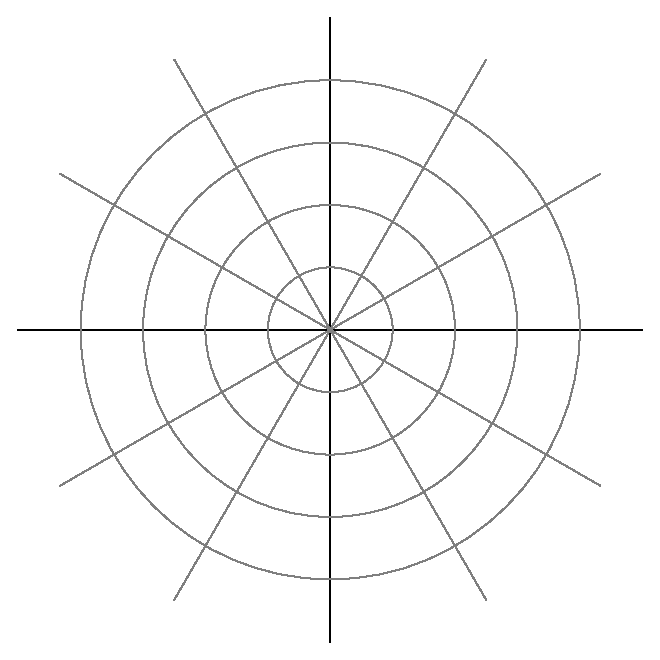
\includegraphics[width=150pt]{polar.eps}
	\end{center}
\vspace*{3in}
\AnswerKeyEntry{The area between the curves is $\frac{\pi}{8}$.}
\end{exercise}

\begin{exercise}{Mixed Practice with Polar Curves \Coffeecup \Coffeecup \Coffeecup}

\begin{itemize}

\item \begin{itemize}
\item Sketch the graph of $r(\theta)=2 \cos(2\theta)$.
	\begin{center}
		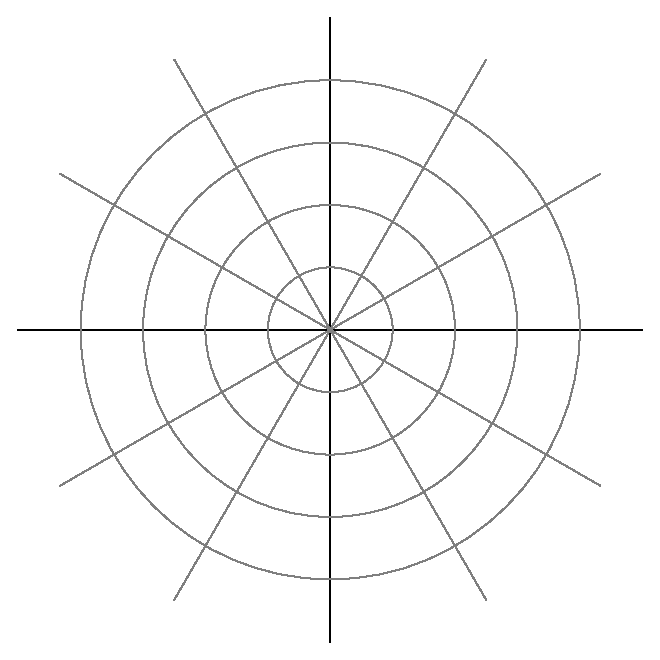
\includegraphics[width=150pt]{polar.eps}
	\end{center}

\item Convert the above curve to cartesian.  That is, find a polynomial equation in $x$ and $y$ whose solution set describes the same set of points.  ({\bf Hint:} Begin by applying the cosine double-angle identity!)

\vspace*{1in}

\end{itemize} 

\item \begin{itemize}
\item  Sketch the graph of  $r(\theta)=\frac{1}{2}+\cos(\theta)$.
	\begin{center}
		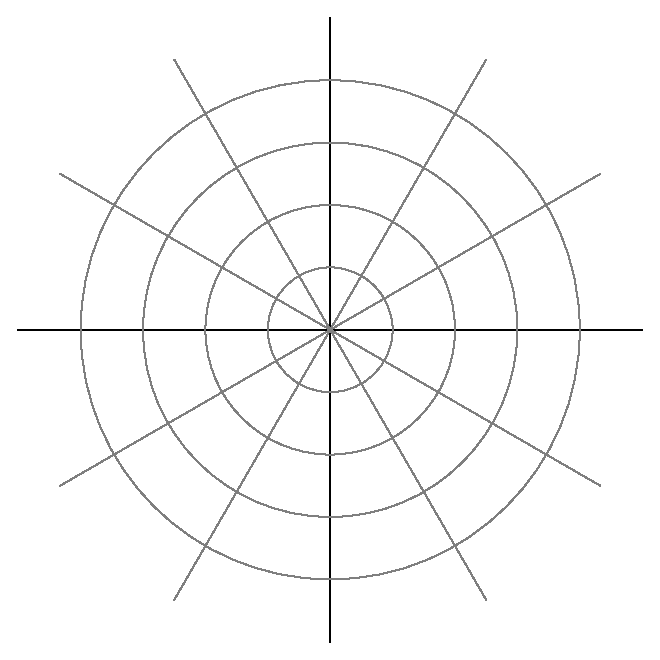
\includegraphics[width=150pt]{polar.eps}
	\end{center}
\item  Find the area enclosed by the inner loop of the graph.
\vspace*{2in}
\AnswerKeyEntry{The area inside the inner loop of $r(\theta)=\frac{1}{2}+\cos(\theta)$ is $\frac{\pi}{4}-\frac{3\sqrt{3}}{8}$.}
\end{itemize}

\item \begin{itemize}
\item  Plot the graphs of both $r_1(\theta)=1+\cos(\theta)$ and $r_2(\theta)=1-\cos(\theta)$ on the same axes.
	\begin{center}
		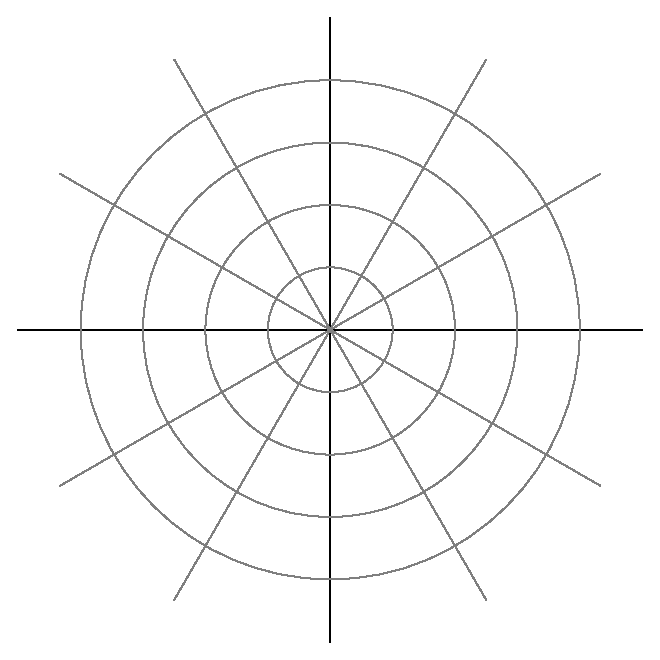
\includegraphics[width=150pt]{polar.eps}
	\end{center}
\item Shade the region contained inside both curves.  Find its area.
\vspace*{2in}
\end{itemize}
\end{itemize}

\end{exercise}

\section{Microphone Design}

A microphone is a device that picks up sound (variations in air pressure) and produces an electrical signal.  For any microphone, sound engineers want what is called the \emph{polar pattern}, a graph indicating all locations from which sound is picked up with equal intensity.  \polar{Microphones} that are physically designed differently will have different polar patterns.

The key element to a microphone is some mechanical device that the waves of air pressure can compress.   There are two basic types of devices:

\subsection{Diaphragm}  A spherical diaphragm responds equally to changes in air pressure from any side.  Thus given a sound of a particular volume, the response in the microphone sensitivity is proportional to the distance from the diaphragm.  A microphone with such a diaphragm is called an \emph{omnidirectional microphone} and is represented by the polar pattern $r(\theta)= 1$, since the microphone has equal sensitivity to all points on a circle.  

\begin{exercise}{Diaphragm Microphones \Coffeecup}
Plot the polar pattern for a diaphragm microphone function below.
	\begin{center}
		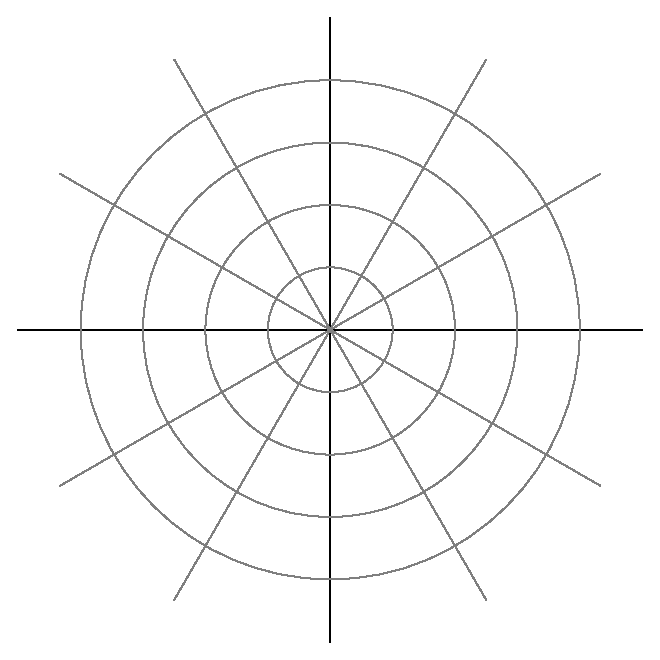
\includegraphics[width=150pt]{polar.eps}
	\end{center}
\end{exercise}

\subsection{Ribbon}
The other main type of device is a ribbon that floats in a magnetic field.  Since it is a horizontal ribbon, it picks up changes in air pressure proportion to the sine of the angle to the source.  (Imagine for example in physics a force pushing on a wall at an angle... the force that goes into the wall is not equal to the magnitude of the whole force but rather the magnitude times sine of the angle.)  A microphone equipped with such a device is called a \emph{ribbon microphone} or a \emph{figure eight microphone} and has polar pattern given by $r(\theta)=\lvert \sin(\theta)\rvert$.  Here we are taking absolute values because we are just denoting sensitivity, not the wave itself.

\begin{exercise}{Ribbon Microphones \Coffeecup \Coffeecup}
Plot the polar pattern for a ribbon microphone function below.
	\begin{center}
		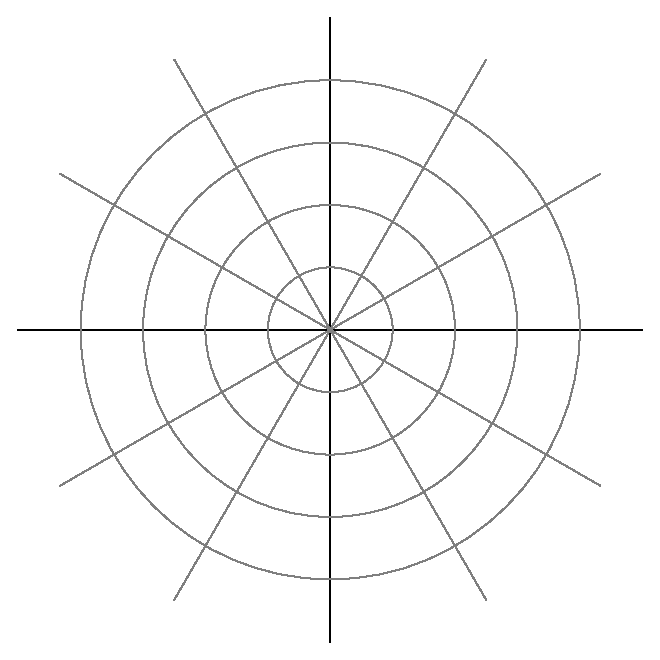
\includegraphics[width=150pt]{polar.eps}
	\end{center}
\end{exercise}

\subsection{Cardioid} 
There are many situations where one of the above microphones is perfect for the purpose at hand.  However, when a band is playing live music on a stage, the above two microphones do not work.  The basic setup is the following: if a singer sings into the microphone, the main speakers are pointed towards the audience and not towards the singer.  Thus, it is necessary to have monitors (smaller speakers pointing the opposite direction) so that the singer can hear herself.  However, if the microphone picks up the sound coming out of the monitor, it's going to be again reproducing the same sound it just heard.  The waves combine amplitude again and again, and this leads to that horrible high-pitched screeching noise known as feedback.  

The solution to this is to design a microphone that picks up sound from one side but not from the other.  The ingenious way engineers figured out how to do this was to simply make a microphone with \emph{both} a ribbon and a diaphragm inside!  The waves produced add to each other to make a single signal.  Thus the sine of the ribbon will combine with the diaphragm's signal on one side, but cancel it out on the other!  The polar pattern is given by the function $r(\theta)=1+\sin(\theta)$ (adding the waves together).  Such a mic is called a \emph{cardioid microphone} and is the standard mic for onstage live sound.  The Shure 57 and Shure 58 are cardioid microphones and have been the standard mic used onstage for about 40 years now!

\begin{exercise}{Cardiod Microphones \Coffeecup \Coffeecup}

\begin{itemize}
\item Plot the polar pattern corresponding to the above described cardioid microphone.
	\begin{center}
		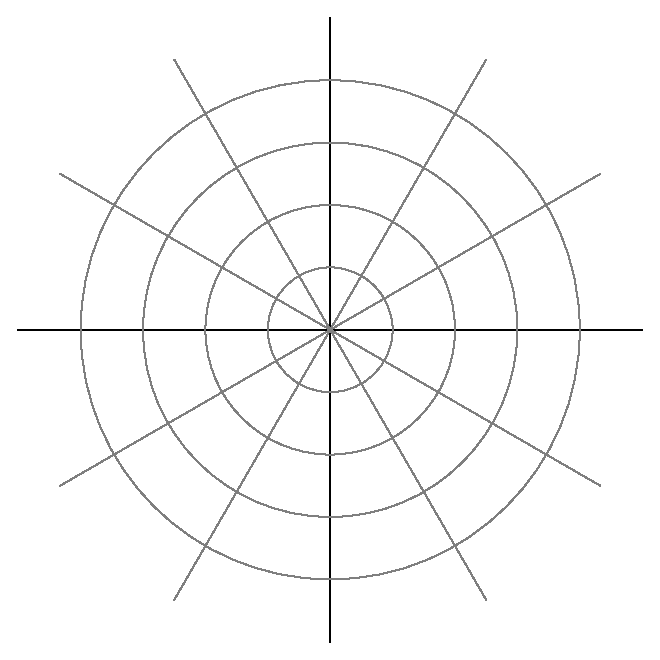
\includegraphics[width=150pt]{polar.eps}
	\end{center}
\item Find the area of the region where sounds are at least as sensitive as they are on the boundary of that cardioid.  (That is, find the area enclosed by the above polar curve.)
\vspace*{2in}
\end{itemize}
\end{exercise}
